% -------------------------------------------------------------------------
% ------ nuweb macros (redefine as desired, or omit with "nuweb -p") ------
% -------------------------------------------------------------------------
\providecommand{\NWtxtMacroDefBy}{Macro defined by}
\providecommand{\NWtxtMacroRefIn}{Macro referenced in}
\providecommand{\NWtxtMacroNoRef}{Macro never referenced}
\providecommand{\NWtxtDefBy}{Defined by}
\providecommand{\NWtxtRefIn}{Referenced in}
\providecommand{\NWtxtNoRef}{Not referenced}
\providecommand{\NWtxtFileDefBy}{File defined by}
\providecommand{\NWsep}{${\diamond}$}
\providecommand{\NWlink}[2]{\hyperlink{#1}{#2}}
\providecommand{\NWtarget}[2]{% move baseline up by \baselineskip 
  \raisebox{\baselineskip}[1.5ex][0ex]{%
    \mbox{%
      \hypertarget{#1}{%
        \raisebox{-1\baselineskip}[0ex][0ex]{%
          \mbox{#2}%
}}}}}
% -------------------------------------------------------------------------

\documentclass[11pt,oneside]{article}	%use"amsart"insteadof"article"forAMSLaTeXformat
\usepackage{geometry}		%Seegeometry.pdftolearnthelayoutoptions.Therearelots.
\geometry{letterpaper}		%...ora4paperora5paperor...
%\geometry{landscape}		%Activateforforrotatedpagegeometry
%\usepackage[parfill]{parskip}		%Activatetobeginparagraphswithanemptylineratherthananindent
%\usepackage{graphicx}				%Usepdf,png,jpg,oreps�withpdflatex;useepsinDVImode
								%TeXwillautomaticallyconverteps-->pdfinpdflatex		
\usepackage{amssymb}
\usepackage[colorlinks=true]{hyperref}
\usepackage{qtree}

%----macros begin-----------------------------------------------------------------------------------
\usepackage{graphicx}
\usepackage{color}
\usepackage{amsthm}

%\renewenvironment{Shaded}{\pause\begin{snugshade}}{\end{snugshade}}
\def\twocolumns#1#2{\begin{columns}
\begin{column}{0.5\linewidth}#1\end{column}
\begin{column}{0.5\linewidth}#2\end{column}
\end{columns}}
\def\mytwocolumns#1#2#3#4{\begin{columns}
\begin{column}{#1\linewidth}#2\end{column}
\begin{column}{#3\linewidth}#4\end{column}
\end{columns}}
\def\mythreecolumns#1#2#3#4#5#6{\begin{columns}
\begin{column}{#1\linewidth}#2\end{column}
\begin{column}{#3\linewidth}#4\end{column}
\begin{column}{#5\linewidth}#6\end{column}
\end{columns}}
\def\threecolumns#1#2#3{\begin{columns}
\begin{column}{0.33\linewidth}#1\end{column}
\begin{column}{0.33\linewidth}#2\end{column}
\begin{column}{0.33\linewidth}#3\end{column}
\end{columns}}
\def\fourcolumns#1#2#3#4{\begin{columns}%
\begin{column}{0.25\linewidth}#1\end{column}%
\begin{column}{0.25\linewidth}#2\end{column}%
\begin{column}{0.25\linewidth}#3\end{column}%
\begin{column}{0.25\linewidth}#4\end{column}%
\end{columns}}

\def\conv{\mbox{\textrm{conv}\,}}
\def\aff{\mbox{\textrm{aff}\,}}
\def\E{\mathbb{E}}
\def\R{\mathbb{R}}
\def\Z{\mathbb{Z}}
\def\tex{\TeX}
\def\latex{\LaTeX}
\def\v#1{{\bf #1}}
\def\p#1{{\bf #1}}
\def\T#1{{\bf #1}}

\def\vet#1{{\left(\begin{array}{cccccccccccccccccccc}#1\end{array}\right)}}
\def\mat#1{{\left(\begin{array}{cccccccccccccccccccc}#1\end{array}\right)}}

\def\lin{\mbox{\rm lin}\,}
\def\aff{\mbox{\rm aff}\,}
\def\pos{\mbox{\rm pos}\,}
\def\cone{\mbox{\rm cone}\,}
\def\conv{\mbox{\rm conv}\,}
\newcommand{\homog}[0]{\mbox{\rm homog}\,}
\newcommand{\relint}[0]{\mbox{\rm relint}\,}

%----macros end-----------------------------------------------------------------------------------


\title{Literate programming IDE for LAR-CC 
\footnote{This document is part of the \emph{Linear Algebraic Representation with CoChains} (LAR-CC) framework~\cite{cclar-proj:2013:00}. \today}
}
\author{Alberto Paoluzzi}
%\date{}							%Activatetodisplayagivendateornodate

\begin{document}
\maketitle
%\nonstopmode

\begin{abstract}
This document introduces the developer of geometric libreries and applications to  the integrated development environment (IDE)  set up for documentation and multilanguage development  using LAR-CC, the Linear Algebraic Representation for geometry, manufacturing and physics with \emph{Chains} and \emph{CoChains}. This IDE is strongly based on the \href{http://www.literateprogramming.com/}{literate programming} tool \emph{Nuweb}, aiming at embedding the code in the documentation, and not vice-versa.
The main goal of this framework is to facilitate how to express the \emph{why} of software design decisions, and not only the tricky details of low level coding.  I would recommend writing programs as if they were research papers and treat the code as you would write mathematical expressions in a research paper. Using multiple programming languages is allowed and even encouraged in \texttt{larcc}. When possible, the same functions coded in different languages should stay close within the same document subsection. The \texttt{larcc} IDE integrates a few programming, documentation and version control tools, including \href{http://www.tug.org/texlive/}{\LaTeX}, \href{http://sourceforge.net/projects/nuweb/}{\emph{Nuweb}}, \href{http://johnmacfarlane.net/pandoc/}{\emph{Pandoc}}, and \href{http://git-scm.com/}{\emph{Git}}.
\end{abstract}

\section{Up and running}

\subsection{Prerequisites}

\paragraph{\LaTeX}
The \texttt{larcc} IDE requires the users to embed the compute code within \LaTeX\ files written for documenting their work. Therefore the first requirement is a working \LaTeX\ environment. ``As \TeX\ Live is the basis of Mac\TeX, and is the \TeX\ system for Unix, if you work cross-platform and want an identical system on all of your machines, then \TeX\ Live is the way to go''~\cite{miktek:2012}.

\paragraph{Python}
As of today, most of \texttt{larcc} development was done in Python. Hence a working Python environment is required, including three packages: \href{http://www.scipy.org}{\texttt{scipy}}, \href{http://pyopengl.sourceforge.net}{\texttt{pyopengl}}, and \href{https://github.com/plasm-language/pyplasm}{\texttt{pyplasm}}. On a Mac, Python is installed by default, whereas \texttt{scipy} and \texttt{pyopengl} may be installed in the terminal by doing 
\begin{verbatim}
$ sudo easy-install scipy
$ sudo easy-install pyopengl
\end{verbatim}
Finally, to install \texttt{pyplasm} look at the README file in its downloaded directory:
\begin{verbatim}
$ git clone https://github.com/plasm-language/pyplasm
\end{verbatim}

\paragraph{Nuweb}

In 1984, Knuth introduced the idea of literate programming. The idea was that a programmer writes just one document, the web file---with suffix \texttt{.w}, that combines the documentation with the code. \emph{Nuweb} works with any programming language and \LaTeX, and is probably the simplest incarnation of the Knut's original work.
The web site of the tool is \href{http://sourceforge.net/projects/nuweb/}{sourceforge.net/projects/nuweb/}.
A revised version of source files can be found on \href{https://code.google.com/p/nuweb/downloads/list}{code.google.com/p/nuweb}. This package can build using the standard tools:
\begin{verbatim}
$ cd <path-to>/nuweb/
$ ./configure
$ make
$ sudo make install
\end{verbatim}
For some documentation read the \href{https://code.google.com/p/nuweb/source/browse/branches/qse-nuweb/README?r=3}{wiki} page.  Test your installation by just compiling to \emph{pdf} the \texttt{nuweb.w} document itself, whose chapter one contains the user documentation:
\begin{verbatim}
$ nuweb nuweb.w
\end{verbatim}
Of course, in order to extend \texttt{larcc} and/or to make an efficient use of it, you are supposed to read carefully the first chapter of the \emph{nuweb.pdf} document.

\subsection{Download}

You may or may not put your IDE under the protection of a version control system. The \texttt{larcc} project comes from \emph{Github} equipped with an integrated \emph{git} system, that you are free either to use or not to use. Of course, my advice  is of making the best use of it. Hence write in the terminal:
\begin{verbatim}
$ git clone https://github.com/cvdlab/larcc
\end{verbatim}

Thats all. Now move to the \texttt{larcc} directory and give a look at its content, a bunch of directories, subdirectories and files, of course. Write
\begin{verbatim}
$ tree -L 2
\end{verbatim}
and you will see something like
\begin{figure}[htbp] %  figure placement: here, top, bottom, or page
   \centering
   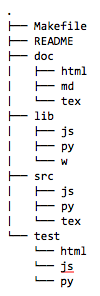
\includegraphics[width=2cm]{images/tree.png} 
   \caption{A sample of the \texttt{larcc} framework}
   \label{fig:tree}
\end{figure}

\subsection{Working-file}
For the impatient, open a terminal, and change directory to \texttt{larcc}, the root of the LAR-CC project, if not already there, whenever you hold it on your system. Then create your working-file \texttt{src/tex/<name>.tex} as a copy of \texttt{src/tex/template.tex}. Open the working-file with an editor, possibly with one aware of the \LaTeX\ syntax, and make few mandatory changes on the template text: 

\begin{description}
\item[Title] change the \texttt{title} command, substituting the ``Title'' string with the actual sentence to be used as document title;
\item[Author]  do the same for the \texttt{author} command, substituting the ``TheAuthor'' string with the actual document author;

\item[Bibliography] substitute the ``template'' string with the actual working-file name (without the file extension).
\end{description}

Finally you may starting the real work by writing the documentation/code within your \texttt{<name>.tex} file, using the simple mark-up rules of \href{run:nuwebdoc.pdf}{Nuweb}.

\subsection{Using the IDE}

In short, in order to use the development environment, you must (a) open your terminal and move to the \texttt{larcc} directory, (b) write a \texttt{tex} file, including documentation and suitably tagged computer code, (c) save it in the \texttt{src} subdirectory, and (d)  execute a \texttt{make} command, asking either for generation of the \texttt{pdf} or the \texttt{html} documentation, or  execution of \href{http://en.wikipedia.org/wiki/Unit_testing}{unit testing}, or simply for the compilation of the source code.


\subsubsection{Using make}

When using the IDE, the user must open the \texttt{Makefile} with any text editor, and modify the current values of two user-definable variables, according to his will:

\begin{verbatim}
NAME = <name>
LANGUAGE = <language>
\end{verbatim}
where \texttt{<name>} is name of the new working document, and \texttt{<language>} may be only \texttt{py} (for Pyton). Soon such values will be extended to include \texttt{<js>} for Javascript and \texttt{<lhs>} for Literate Haskell.
The make \emph{targets} currently available in the Makefile are the following:
\begin{description}
\item[all] 
is the default option. Its execution produces a \emph{pdf} document in the \texttt{doc/pdf} subdirectory, and a pair of \emph{tex}/\emph{bbl} documents in the \texttt{doc/tex} subdirectory, all using name \texttt{<name>};
\item[html] 
similar to the default option, but produces a directory named \texttt{<name>} wth a bunch of \emph{html} pages, located in the \texttt{doc/html} subdirectory;

\item[test] 
to execute the tests contained in the directory \texttt{test/<language>/<name>}
\item[exec] 
to execute \emph{nuweb} on the working document, i.e.~on \texttt{<name>.tex}\footnote{Actually, \texttt{<name>.tex} is internally copied to a scratch file \texttt{<name>.w}, in order to allow the user to work comfortably with an editor knowledgeable of the \LaTeX\ syntax.}; this execution generates both the \LaTeX\ documentation file and the source output files (for example the unit tests) written in the coding \texttt{<language>};
\item[clear] 
to remove all the working files from the root directory. Used by other commands. To be invoked by the user just in case that something did not work out.
\end{description}



\section{Structure of \texttt{larcc}}

The \texttt{larcc} project is hinged around four subdirectories (see Figure~\ref{fig:tree}) and a Makefile.
The meaning and function of the four subdirectories are listed below.

\begin{description}
\item[src]  (for \emph{Source})
is the directory \texttt{src}  that contains all the source documents, and in particular the \texttt{tex} files including the code of the algorithms and the tests developed in the project. It is divided in subdirectories related to the type of the source file itself. For example a \texttt{html} directory will contain the user-defined \texttt{css} source files, and the \texttt{lhs} directory the \emph{literate Haskell} sorce files, to be processed directly by the Haskell compiler \emph{GHC}.
Such directories will also contain other programming resources needed to build the libreries or the applications developed in the LAR-CC project.

\item[test] 
\href{http://en.wikipedia.org/wiki/Test-driven_development}{test-driven development} (TDD) is a software development process that relies on the repetition of a very short development cycle: write a ``unit test'', get it to pass, run all tests, clean up the code (see Figure~\ref{fig:tdd}).
The subdirectory \texttt{test} is the repository of test suites, collection of test cases, and of unit test files, possibly grouped depending on the source language, to be launched either individually, while writing each single software function or application, or collectively before committing or pushing novel developments or subsystems. 

\item[lib] 
is the repository of compiled and/or executable programs. In particular, it is the place where to store and retrieve all the libreries or modules or applications developed by compilation of any  document within the \texttt{scr} subdirectory of the \texttt{larcc} system, excluding the documentation.

\item[doc] 
conversely contains all the documentation generated by the system, once again subdivided depending on the language and tools used for its reading or examination.
\end{description}

\begin{figure}[htbp] %  figure placement: here, top, bottom, or page
   \centering
   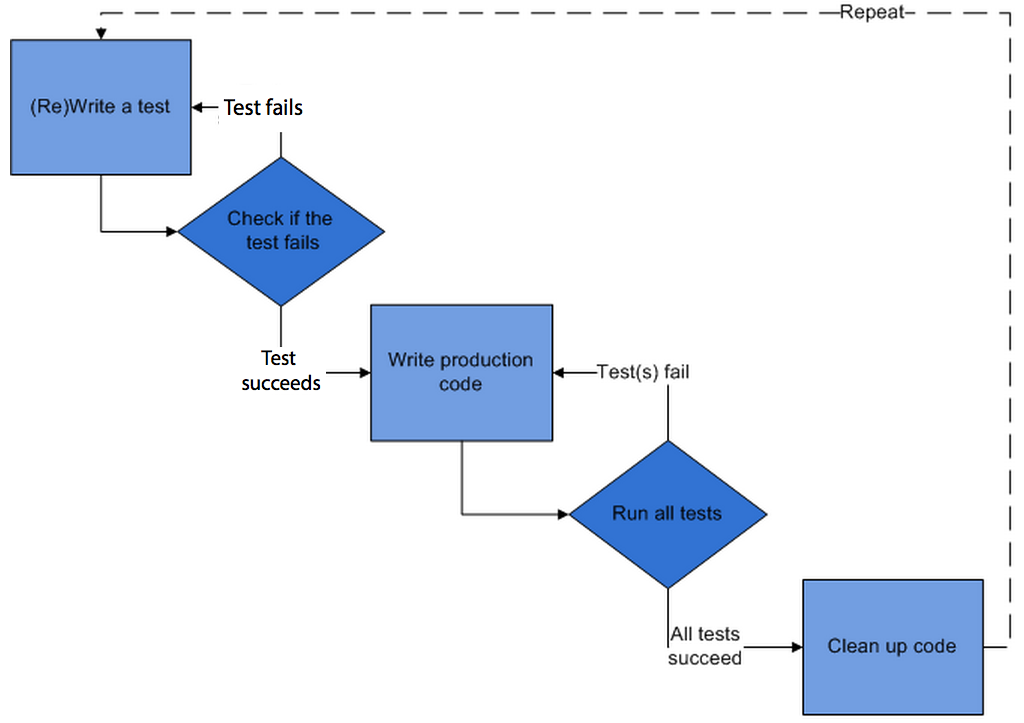
\includegraphics[width=0.8\linewidth]{images/tdd.png} 
   \caption{test-driven development (TDD) cycle (from Wikipedia)}
   \label{fig:tdd}
\end{figure}

\bibliographystyle{amsalpha}
\bibliography{framework}

\end{document}
